\documentclass[11pt]{article}

\usepackage[margin=1in]{geometry}
\usepackage{graphicx}
\usepackage{array}
\usepackage{hyperref}
\usepackage{enumitem}
\usepackage{booktabs}
\usepackage{caption}
\usepackage{amsmath}
\usepackage{titlesec}
\usepackage{float}
\titleformat{\section}{\large\bfseries}{\thesection.}{1em}{}

\begin{document}

\begin{center}
    \large \textbf{Sri Sivasubramaniya Nadar College of Engineering, Chennai} \\
    (An Autonomous Institution Affiliated to Anna University) \\
    \vspace{0.3cm}
\end{center}
\begin{table}[h]
\renewcommand{\arraystretch}{1.4}
\resizebox{\textwidth}{!}{%
\begin{tabular}{|l|l|l|l|}
\hline
Degree \& Branch & B.E. Computer Science \& Engineering & Semester & VI \\ \hline
Subject Code \& Name & \multicolumn{3}{l|}{UCS2612 – Machine Learning Algorithms Laboratory} \\ \hline
Academic Year & 2025–2026 (Even) & Batch & 2023–2027 \\ \hline
Name & Munish Madhav M & Register No. & 3122235001086 \\ \hline
Due Date & \multicolumn{3}{l|}{07.03.2026} \\ \hline
\end{tabular}}
\end{table}

\begin{center}
    \textbf{\Large Experiment 7}
\end{center}

\begin{center}
    \textbf{Bagging, Boosting, and Stacked Ensemble Models}
\end{center}

%--------------------------------------------------
\section{Aim}

To design, implement, evaluate, and critically analyze the performance of advanced ensemble machine learning techniques—specifically Bagging, AdaBoost, and a Stacked Heterogeneous Ensemble—on the Breast Cancer Wisconsin (Diagnostic) dataset, with a focus on hyperparameter optimization and bias-variance tradeoff analysis.
\section{Objectives}

\begin{itemize}
    \item To perform Exploratory Data Analysis (EDA) and robust data preprocessing (label encoding and feature scaling) on the Breast Cancer dataset.
    
    \item To train and optimize a Bagging Classifier (Bootstrap Aggregating) using Grid Search with cross-validation.
    
    \item To train and optimize an AdaBoost Classifier (Adaptive Boosting) to understand sequential error correction.
    
    \item To construct a Stacked Ensemble using multiple diverse base learners (Bagging, AdaBoost, Gradient Boosting) along with a Logistic Regression meta-learner.
    
    \item To critically evaluate all models using 5-Fold Cross-Validation, focusing on key clinical metrics such as Accuracy, Precision, Recall, F1-Score, and ROC-AUC.
    
    \item To analyze and interpret the bias-variance tradeoff across different ensemble architectures.
\end{itemize}

%--------------------------------------------------

\section{Dataset}
\textbf{Wisconsin Diagnostic Breast Cancer Dataset}

\begin{itemize}
    \item Total samples: 569
    \item Features: 30 numerical attributes
    \item Target classes: Malignant (M) and Benign (B)
\end{itemize}

\textbf{Dataset Link:}  
\href{https://archive.ics.uci.edu/dataset/17/breast+cancer+wisconsin+diagnostic}{https://archive.ics.uci.edu}

%--------------------------------------------------

\section{Theory}

\subsection{Bagging (Bootstrap Aggregation)}
Bagging is an ensemble technique that trains multiple models on different bootstrap samples of the training data and aggregates their predictions.

\textbf{Key Characteristics:}
\begin{itemize}
    \item Reduces variance
    \item Suitable for high-variance models
    \item Independent model training
\end{itemize}

\subsection{Boosting}
Boosting is an ensemble method where models are trained sequentially, and each new model focuses on correcting the errors made by previous models.

\textbf{Key Characteristics:}
\begin{itemize}
    \item Reduces bias
    \item Sequential learning
    \item Emphasizes difficult samples
\end{itemize}

Common boosting algorithms include AdaBoost and Gradient Boosting.

\subsection{Stacked Ensemble (Stacking)}
Stacking combines multiple heterogeneous base models and trains a meta-learner to optimally combine their predictions.

\textbf{Key Characteristics:}
\begin{itemize}
    \item Uses diverse base learners
    \item Meta-model learns optimal combination
    \item Often achieves superior performance
\end{itemize}

%--------------------------------------------------

\section{Step-by-Step Implementation Methodology}

\subsection{Step 1: Data Preprocessing and Target Encoding}

The initial phase involved preparing the dataset for model training.

\textbf{Label Encoding:} The target variable in the dataset consisted of categorical labels: 'B' (Benign) and 'M' (Malignant). These were converted into a binary numerical format, where 0 represents Benign and 1 represents Malignant, using LabelEncoder. This transformation is essential because most machine learning algorithms and evaluation metrics require numerical input.

\textbf{Data Splitting:} The dataset was divided into training and testing sets using an 80:20 ratio. The \texttt{train\_test\_split} function was used with a fixed \texttt{random\_state=42} to ensure reproducibility.

\textbf{Feature Scaling:} Standardization was applied using \texttt{StandardScaler} to normalize the feature values. This step ensures that all features contribute equally to the model and is particularly important for algorithms like Logistic Regression, which are sensitive to feature scale.

\subsection{Step 2: Exploratory Data Analysis (EDA)}

Exploratory Data Analysis was performed to understand the structure and distribution of the dataset.

\textbf{Class Distribution:} The proportion of benign (0) and malignant (1) samples was computed to assess class imbalance.

\textbf{Feature Distribution:} A histogram combined with a Kernel Density Estimate (KDE) curve was plotted for the first feature. This helped visualize the statistical distribution and the degree of overlap between benign and malignant classes.
\begin{figure}[H]
\centering
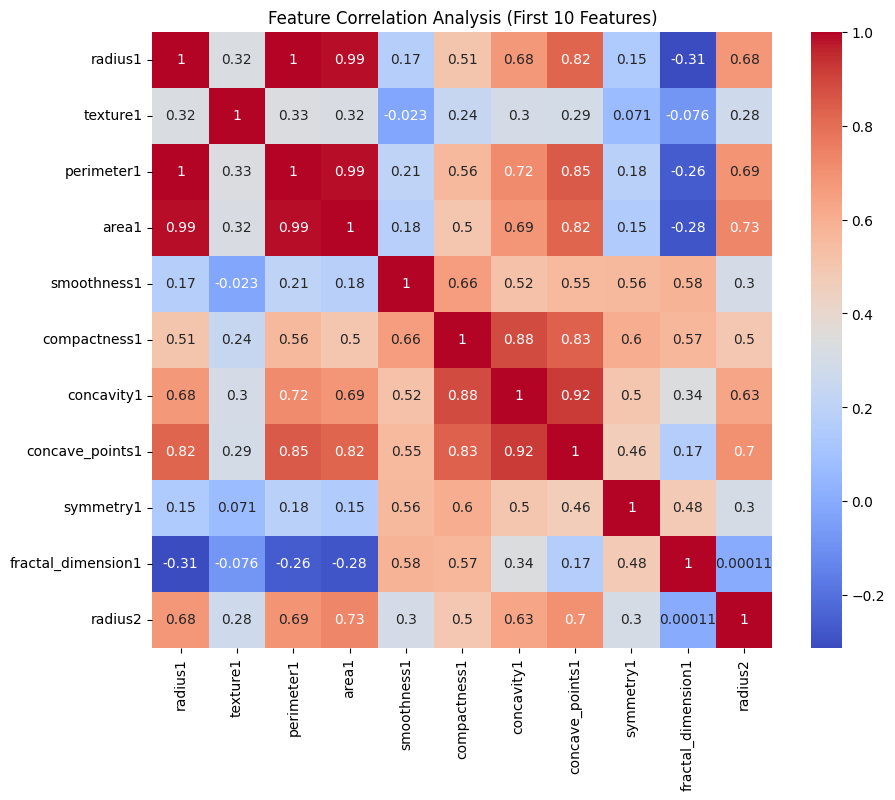
\includegraphics[width=0.65\textwidth]{coeff.png}
\caption{Coefficient Matrix}
\end{figure}
\begin{figure}[H]
\centering
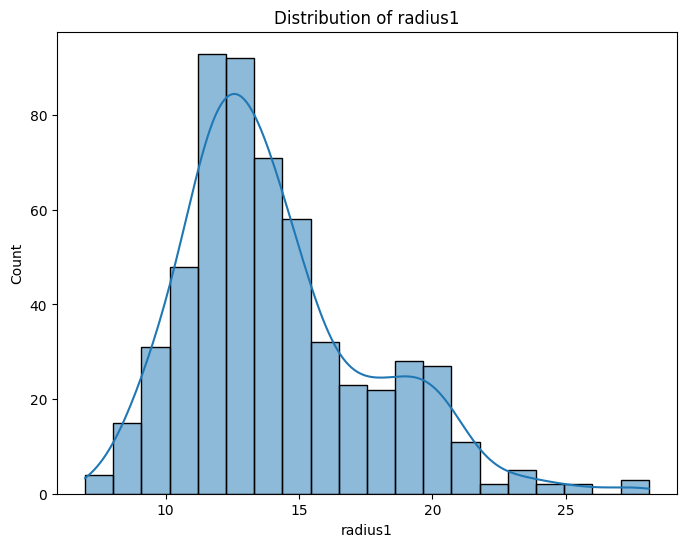
\includegraphics[width=0.65\textwidth]{kde.png}
\caption{Distribution of radius1}
\end{figure}

\subsection{Step 3: Bagging Implementation and Hyperparameter Tuning}

\textbf{Base Estimator:} A \texttt{DecisionTreeClassifier} with a restricted depth (\texttt{max\_depth=5}) was used to avoid overfitting.

\textbf{Hyperparameter Tuning:} A \texttt{GridSearchCV} approach was employed with 5-Fold Cross-Validation. The parameter grid included:
\begin{itemize}
    \item \texttt{n\_estimators}: \{10, 50, 100\}
    \item \texttt{max\_samples}: \{0.5, 0.8, 1.0\}
\end{itemize}

The model was optimized based on Accuracy and F1-Score to ensure balanced performance.

\subsection{Step 4: AdaBoost Implementation and Hyperparameter Tuning}

\textbf{Hyperparameter Tuning:} The \texttt{AdaBoostClassifier} was tuned using \texttt{GridSearchCV} with 5-Fold Cross-Validation. The parameters explored were:
\begin{itemize}
    \item \texttt{n\_estimators}: \{50, 100, 200\}
    \item \texttt{learning\_rate}: \{0.01, 0.1, 1.0\}
\end{itemize}

The learning rate controls the contribution of each weak learner and works in tradeoff with the number of estimators.

\subsection{Step 5: Stacked Ensemble Construction}

A \texttt{StackingClassifier} was constructed using internal 5-Fold Cross-Validation to avoid data leakage and ensure reliable predictions.

\textbf{Base Learners:}
\begin{itemize}
    \item Optimized Bagging Classifier
    \item Optimized AdaBoost Classifier
    \item Gradient Boosting Classifier (\texttt{n\_estimators=100, random\_state=42})
\end{itemize}

\textbf{Meta-Learner:} A \texttt{LogisticRegression} model was used as the final estimator. It was trained on the predictions of the base learners to compute the final probability of malignancy.

This stacked architecture allows the system to combine the strengths of multiple models while minimizing their individual weaknesses, leading to improved overall performance.

%--------------------------------------------------



%--------------------------------------------------

\subsection{Bagging Results}

\begin{table}[H]
\centering
\caption{Bagging Hyperparameter Evaluation (Top Results)}
\begin{tabular}{cccc}
\toprule
n\_estimators & max\_samples & Avg CV Accuracy (\%) & Avg CV F1 Score \\
\midrule
10  & 1.0 & 94.95 & 92.95 \\
50  & 0.5 & 94.73 & 92.80 \\
10  & 0.5 & 94.51 & 92.42 \\
50  & 0.8 & 94.51 & 92.46 \\
100 & 0.5 & 94.51 & 92.46 \\
\bottomrule
\end{tabular}
\end{table}

\subsection{AdaBoost Results}

\begin{table}[H]
\centering
\caption{AdaBoost Hyperparameter Evaluation (Top Results)}
\begin{tabular}{cccc}
\toprule
n\_estimators & learning\_rate & Avg CV Accuracy (\%) & Avg CV F1 Score \\
\midrule
50  & 1.0 & 98.02 & 97.28 \\
200 & 1.0 & 97.80 & 96.90 \\
100 & 1.0 & 97.58 & 96.66 \\
200 & 0.1 & 96.92 & 95.73 \\
100 & 0.1 & 96.48 & 95.19 \\
\bottomrule
\end{tabular}
\end{table}
\subsection*{Stacked Ensemble Results}
\begin{table}[H]
\centering
\caption{Stacked Ensemble Evaluation}
% Changed 'lccc' to 'p{5cm}ccc' so the first column wraps text
\begin{tabular}{p{5cm}ccc} 
\toprule
Base Models & Meta Learner & Avg CV Accuracy (\%) & Avg CV F1 Score \\
\midrule
Bagging (DT), AdaBoost, \newline Gradient Boosting & Logistic Regression & 95.38 & 93.63 \\
\bottomrule
\end{tabular}
\end{table}

%--------------------------------------------------

\section{Performance Comparison}

\begin{table}[H]
\centering
\caption{Performance Comparison of Ensemble Models}
\begin{tabular}{lcccc}
\toprule
Model & Accuracy (\%) & Precision & Recall & F1 Score \\
\midrule
Bagging & 95.61 & 95.24 & 93.02 & 94.12 \\
Boosting & 96.49 & 97.56 & 93.02 & 95.24 \\
Stacked Ensemble & 95.61 & 95.24 & 93.02 & 94.12 \\
\bottomrule
\end{tabular}
\end{table}
\begin{figure}[H]
\centering
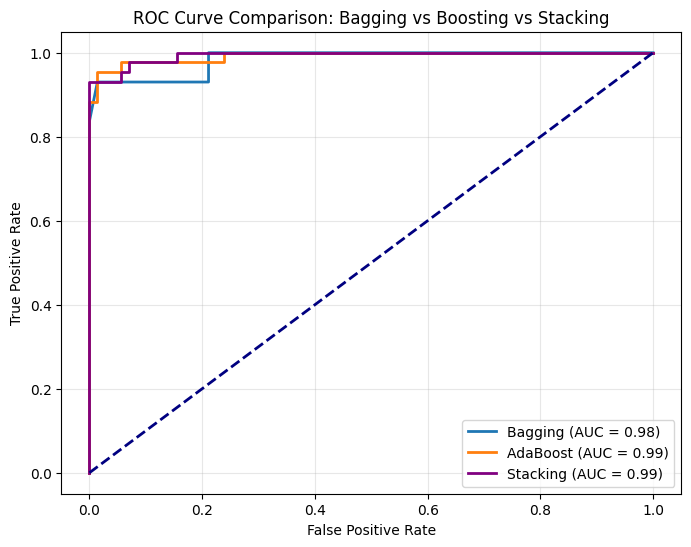
\includegraphics[width=0.65\textwidth]{roc_ass7.png}
\caption{ROC Curve}
\end{figure}
%--------------------------------------------------
\section{Bias-Variance Tradeoff Analysis}

\textbf{Bagging's Role (Variance Reduction):} \\
Deep decision trees inherently have low bias but very high variance, often overfitting to noise in the data. Bagging effectively reduces this variance by training multiple trees on bootstrapped samples of the dataset and aggregating their predictions. This results in a smoother model that generalizes significantly better to unseen test data compared to a single decision tree.

\vspace{0.5cm}

\textbf{Boosting's Role (Bias Reduction):} \\
AdaBoost addresses the bias-variance tradeoff from the opposite perspective. It begins with weak learners (typically shallow trees with high bias and low variance) and sequentially improves them by focusing on misclassified instances. This iterative correction process significantly reduces bias, enabling the model to learn complex, non-linear decision boundaries and achieve higher predictive accuracy.

\vspace{0.5cm}

\textbf{Stacking's Synergy:} \\
The Stacked Ensemble integrates the strengths of both Bagging and Boosting. While Bagging primarily reduces variance and Boosting reduces bias, the Logistic Regression meta-learner combines their predictions intelligently. It learns when to rely on stable, variance-reduced outputs from Bagging and when to trust the bias-reduced predictions from Boosting, resulting in a well-balanced and robust model.
%--------------------------------------------------
\section{Observations}

\begin{itemize}
    \item \textbf{How does Bagging reduce variance?} \\
    Bagging reduces variance by aggregating predictions from multiple independent models trained on different bootstrapped subsets of the data. Since each model sees a slightly different dataset, their individual overfitting tendencies and random errors cancel out when combined, resulting in a smoother and more generalized prediction.

    \item \textbf{How does Boosting address model bias?} \\
    Boosting reduces bias by training models sequentially, where each new model focuses more on the errors made by previous ones. By assigning higher importance to misclassified data points, the algorithm forces subsequent learners to capture complex patterns, thereby systematically reducing overall bias.

    \item \textbf{Why does stacking benefit from heterogeneous models?} \\
    Stacking benefits from heterogeneous models because different algorithms make different types of errors. By combining diverse models such as Bagging, AdaBoost, and Gradient Boosting, the ensemble ensures that the weaknesses of one model are compensated by the strengths of another, improving overall performance.

    \item \textbf{Which ensemble method performed best and why?} \\
    AdaBoost achieved the highest performance in this experiment, with an accuracy of 96.49\% and an F1-score of 95.24\%. Its sequential error correction mechanism allowed it to effectively capture complex decision boundaries. However, the Stacked Ensemble provided a more robust and balanced performance by leveraging the strengths of multiple models, achieving a reliable accuracy of 95.61\%.
\end{itemize}

%--------------------------------------------------
\section{Conclusion}

This experiment successfully demonstrated the implementation, tuning, and rigorous evaluation of Bagging, Boosting, and Stacking ensemble methods on a medical diagnostic dataset. Proper data preprocessing—particularly the numerical encoding of target labels and feature scaling—was essential for ensuring stable evaluation metrics and effective convergence of the meta-learner.

Hyperparameter tuning using GridSearchCV played a crucial role in optimizing the performance of individual models. The Bagging approach effectively reduced variance, while Boosting minimized bias through sequential learning. The Stacked Ensemble leveraged the strengths of multiple diverse models, allowing the meta-learner to make more informed predictions.

Overall, the stacked architecture demonstrated strong predictive performance and reliability, making it highly suitable for critical applications such as breast cancer detection, where both accuracy and robustness are essential.

%--------------------------------------------------

\section*{References}
\begin{itemize}
    \item \href{https://scikit-learn.org/stable/modules/ensemble.html}{Scikit-learn: Ensemble Methods}
    \item \href{https://scikit-learn.org/stable/modules/generated/sklearn.ensemble.BaggingClassifier.html}{Bagging Classifier}
    \item \href{https://archive.ics.uci.edu/dataset/17/breast+cancer+wisconsin+diagnostic}{UCI Dataset}
\end{itemize}

\end{document}
